%%%%%%%%%%%%%%%%%%%%%%%%%%%%%%%%%%%%%%%%%%%%%%%%%%%%%%%%%%%%%%%%%%%%%%
% LaTeX Example: Project Report
%
% Source: http://www.howtotex.com
%
% Feel free to distribute this example, but please keep the referral
% to howtotex.com
% Date: March 2011 
% 
%%%%%%%%%%%%%%%%%%%%%%%%%%%%%%%%%%%%%%%%%%%%%%%%%%%%%%%%%%%%%%%%%%%%%%
% How to use writeLaTeX: 
%
% You edit the source code here on the left, and the preview on the
% right shows you the result within a few seconds.
%
% Bookmark this page and share the URL with your co-authors. They can
% edit at the same time!
%
% You can upload figures, bibliographies, custom classes and
% styles using the files menu.
%
% If you're new to LaTeX, the wikibook is a great place to start:
% http://en.wikibooks.org/wiki/LaTeX
%
%%%%%%%%%%%%%%%%%%%%%%%%%%%%%%%%%%%%%%%%%%%%%%%%%%%%%%%%%%%%%%%%%%%%%%
% Edit the title below to update the display in My Documents
%\title{Project Report}
%
%%% Preamble
\documentclass[paper=letter, fontsize=10pt]{scrartcl}
\usepackage[body={7in,7.5in},top=1in, bottom=1in]{geometry}
\usepackage[T1]{fontenc}
\usepackage{fourier}

\usepackage[english]{babel}															% English language/hyphenation
\usepackage[protrusion=true,expansion=true]{microtype}	
\usepackage{amsmath,amsfonts,amsthm} % Math packages
\usepackage[pdftex]{graphicx}	
\usepackage{url}
\usepackage{enumerate}
\usepackage{lastpage}


%%% Custom sectioning
\usepackage{sectsty}
\allsectionsfont{\normalfont\scshape}


%%% Custom headers/footers (fancyhdr package)
\usepackage{fancyhdr}
\pagestyle{fancy}
\fancyhead[L]{}
\fancyhead[c]{Requirements Revision 0}
\fancyhead[R]{\today}											
\fancyfoot[L]{}											 
\fancyfoot[C]{}											
\fancyfoot[R]{\thepage\ of \pageref{LastPage}}		% Pagenumbering
\renewcommand{\headrulewidth}{0.4pt}				% Remove header underlines
\renewcommand{\footrulewidth}{0.4pt}				% Remove footer underlines
\setlength{\headheight}{13.6pt}


%%% Equation and float numbering
\numberwithin{equation}{section}		% Equationnumbering: section.eq#
\numberwithin{figure}{section}			% Figurenumbering: section.fig#
\numberwithin{table}{section}				% Tablenumbering: section.tab#


%%% Maketitle metadata
\newcommand{\horrule}[1]{\rule{\linewidth}{#1}} 	% Horizontal rule
\newcommand{\ts}{\textsuperscript}

%%% Begin document
\begin{document}

\begin{titlepage}

\newcommand{\HRule}{\rule{\linewidth}{0.5mm}} % Defines a new command for the horizontal lines, change thickness here

\begin{center}
 
%----------------------------------------------------------------------------------------
%	HEADING SECTIONS
%----------------------------------------------------------------------------------------

\textsc{\LARGE McMaster University}\\[1.5cm] % Name of your university/college
\textsc{\Large CAS 4ZP6 Capstone Project 2013/2014}\\[0.5cm] % Major heading such as course name
\textsc{\large Porter Simulation}\\[0.5cm] % Minor heading such as course title

%----------------------------------------------------------------------------------------
%	TITLE SECTION
%----------------------------------------------------------------------------------------

\HRule \\[0.4cm]
{ \huge \bfseries User Manual Revision 0}\\[0.4cm] % Title of your document
\HRule \\[1.5cm]
 
%----------------------------------------------------------------------------------------
%	AUTHOR SECTION
%----------------------------------------------------------------------------------------

\begin{minipage}{0.4\textwidth}
\begin{flushleft} \large
\emph{Authors:}\\
Vitaliy Kondratiev - 0945220\\
Nathan Johrendt - 0950519\\
Tyler Lyn - 0948978\\
Mark Gammie - 0964156
\end{flushleft}
\end{minipage}
~
\begin{minipage}{0.4\textwidth}
\begin{flushright} \large
\emph{Supervisor:} \\
Dr. Douglas Down % Supervisor's Name
\end{flushright}
\end{minipage}\\[4cm]

% If you don't want a supervisor, uncomment the two lines below and remove the section above
%\Large \emph{Author:}\\
%John \textsc{Smith}\\[3cm] % Your name

%----------------------------------------------------------------------------------------
%	DATE SECTION
%----------------------------------------------------------------------------------------

{\large \today}\\[3cm] % Date, change the \today to a set date if you want to be precise

%----------------------------------------------------------------------------------------
%	LOGO SECTION
%----------------------------------------------------------------------------------------

%\includegraphics{Logo}\\[1cm] % Include a department/university logo - this will require the graphicx package
 
%----------------------------------------------------------------------------------------

\vfill % Fill the rest of the page with whitespace
\end{center}
\end{titlepage}

\setcounter{tocdepth}{2}

\tableofcontents

\newpage
\section{Introduction}
Welcome to the User Manual for the Hamilton Health Science's Porter Simulation, designed for use at the Juravinski Hospital in Hamilton Ontario. This manual will guide a Hamilton Health Science professional through the functions and features available when using the simulation software. In addition, this manual will provide you steps for software setup, an overview of the configuration settings (user interface) and provide troubleshooting options should any issues arise.

\section{Installation}
Setup of the Porter Simulation is quick and easy, by following these steps the software will be accessible for use.  This software is designed to be installed on Windows XP/Vista/7/8.
\begin{enumerate}
	\item Locate the Porter Simulation folder on your computer. This folder will be located on a USB removable device, CD or through an email download.
	\item Inside the folder, double click to run the Porter Simulation-0.1-win32.msi
	\item Pick a directory to install the application. Default directory will be automatically filled in
	\item Wait for the installer to finish then click "Finish"
	\item The Porter Simulation shortcut will now appear on your desktop where it can be accessed
\end{enumerate}

\begin{figure}[!htbp]
	\begin{center}
		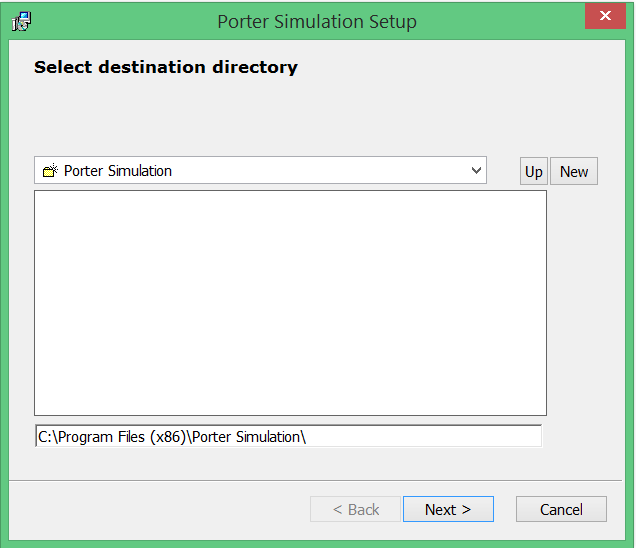
\includegraphics[width=1\columnwidth, height=0.5\textheight, keepaspectratio]{Installer.png}
		\caption{Pick a directory}
	\end{center}
\end{figure}

\section{Input Configuration}
The first step in using the software is to configure the simulation with a series of different inputs. These different input variables represent changes to the hospital environment, which will affect the simulated results.

	\begin{figure}[!htbp]
	\begin{center}
		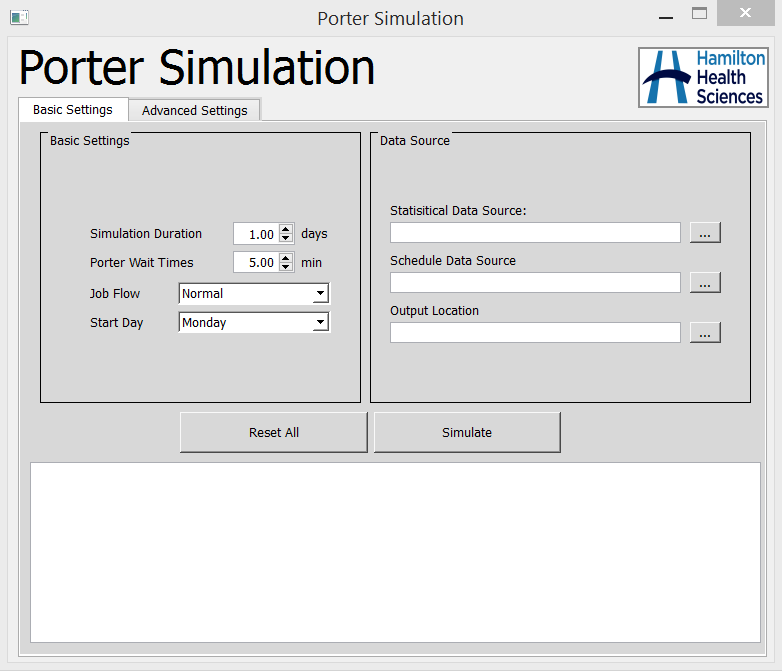
\includegraphics[width=1\columnwidth, height=0.5\textheight, keepaspectratio]{BasicSettings.png}
		\caption{Basic Settings}
	\end{center}
	\end{figure} 
	\subsection{Basic Settings - General}
	These general settings define base values for the simulation.
	\begin{enumerate}[(i)]
		\item \textbf{Number of Porters:} Defines how many individual porters are working in the simulated hospital.
		\item \textbf{Job Distribution:} Jobs are added to a pool for available porters to receive. This setting allows the volume and frequency of jobs to be adjusted.
		\item \textbf{Simulation Duration:} The number of hours or days the software will simulate. Note that this is not how long the simulation will run, but how much time will be modeled virtually by the software. 
	\end{enumerate}
	
	\subsection{Basic Settings - Compliance}
	Compliance settings reflect the performance of the virtual porters and modify how they will react to situations in the hospital.
	\begin{enumerate}[(i)]
		\item \textbf{Correct Equipment Usage:} The frequency at which jobs encounter no delays from improper equipment use or management.
		\item \textbf{Patient Readiness:} The frequency at which patients are prepared for transport immediately when a porter arrives to pick them up for a job.
		\item \textbf{Porter Wait Times:} This variable represents how long on average porters will wait for a patient who is not ready. Handy for testing variations on the 5 and 5 compliance rule.
		\item \textbf{Chance of Job Cancellation:} The frequency that a porter will cancel a job after waiting too long for patient that is not ready. This job is then re-entered into the job pool to be dispatched again.
	\end{enumerate}
	
	\subsection{Basic Settings - Data Source}
	The Data Source setting allows selection of different source input files, pre-configured to aid HHS users in testing a variety of hospital conditions and elements. 
	\begin{enumerate}[(i)]
		\item \textbf{Use Data From:} Allows selection of a timeframe that the simulation will sample job information from.
		\item \textbf{Statistical Data Source:} Determines which source file will be used to provide the simulation with statistical distribution information. 
		\item \textbf{Schedule Data Source:} This variable will determine the method of porter scheduling that the simulation will model, allowing variation in porter shift times, staffing levels and break management.
	\end{enumerate}
	
	\subsection{Advanced Settings - Dispatcher}
	The dispatcher will be ordering the pending jobs and giving them to available porters.  These settings reflect the current dispatcher system at Jurvinski Hospital.
	
	\begin{figure}[!htbp]
	\begin{center}
		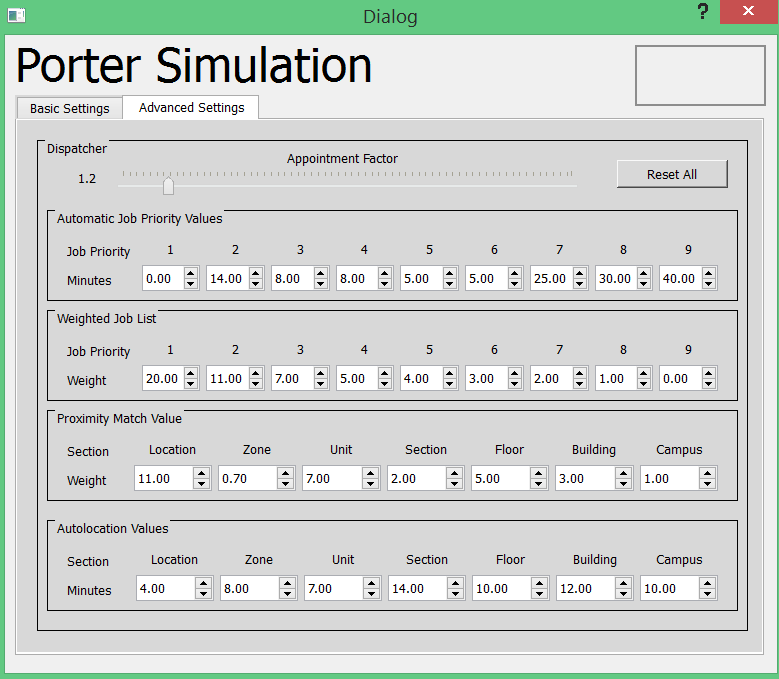
\includegraphics[width=1\columnwidth, height=0.48\textheight, keepaspectratio]{AdvancedSettings.png}
		\caption{Advanced Settings}
	\end{center}
	\end{figure} 
	\begin{enumerate}[(i)]
		\item \textbf{Appointment Factor:} Jobs that are scheduled in advanced need to be given priority over jobs generated on-demand.  Increasing the appointment factor will decrease the time scheduled jobs spend waiting for a porter.
		\item \textbf{Automatic Job Priority Values:} Jobs waiting for a porter need to increase their priority after waiting for a specified amount of time.  The "Minutes" will determine how long a job waits until it increases in priority.
		\item \textbf{Weighted Job List:} Jobs of different priorities need to have different weights.  This weight helps determine how quickly the job should be assigned to a porter.
		\item \textbf{Proximity Match Values:} The closeness of a porter to pending jobs will factor into how quickly a job is assigned to a porter.
	\end{enumerate}
	
	\subsection{Porter Schedule}
	Porters need to be scheduled by shifts in order to give the users flexibility over the simulation.  This will allow the user full control over the amount of porters available over the course of a simulation.
	
	\begin{figure}[!htbp]
	\begin{center}
		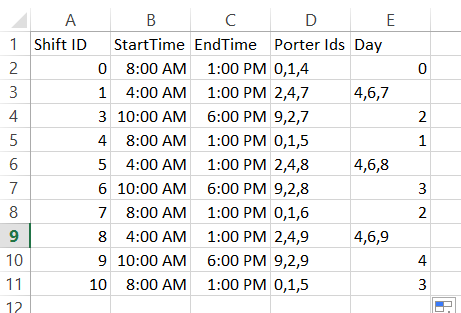
\includegraphics[width=1\columnwidth, height=0.5\textheight, keepaspectratio]{Schedule.png}
		\caption{Porter Schedule}
	\end{center}
	\end{figure}
	
	\begin{enumerate}[(i)]
		\item \textbf{Shift ID:} An identifier for a shift.  The Shift ID will allow for the easier of traceability of shifts in the output data.
		\item \textbf{StartTime:} A shift will begin at this time in the simulation.
		\item \textbf{EndTime:} A shift will end at this time in the simulation.
		\item \textbf{Porters Ids:} Allows for the assignment of one or more porter(s) to a shift.  A porter is assigned to a shift by adding an identifier.  Multiple porters can be assigned to the same shift by adding multiple identifiers each separated by a comma.  In the Figure 3.3 \textit{Shift ID 0} has three  porters assigned to it \textit{0,1,4}.
		\item \textbf{Day:} The day of the week on which the shift occurs.  It must be a number from 1-7, 1 being Monday and 7 being Sunday.
	\end{enumerate}
\section{Output Data}
Once the simulation has finished modeling and computing the data, the results of all of the completed jobs are exported to an excel file. This file contains some graphs and plots, as well as some data averages to better analyze the simulated results. The file is located in the same directory as PorterSimulation.exe. While the existing plots will be beneficial in interpreting the resulting output, users are encouraged to explore their data using the tools built into excel. Details on the specific graphs and data layout will be available once development is complete.

\section{Troubleshooting}
The Porter Simulation has been designed to operate effectively and error free, however, this troubleshooting section will help address any minor issues that may arise.

\begin{enumerate}[(i)]
	\item \textbf{Simulation Stops:} In the event that the simulation is running and suddenly halts before producing output data, it will be necessary to close the simulation manually by clicking the X in the top right corner of the window. If the simulation continues to malfunction, please contact the development team.
	\item \textbf{Data Files Missing:} When selecting source data files, if the files do not appear in the listings on the Basic Settings screen, check the Porter Simulation installation directory. If the files are missing, they can easily be added again by copying them from the Porter Simulation installer package, either by download or from USB storage.
\end{enumerate}

\section{Figures and Tables Appendix}
\begin{enumerate}[(a)]
	\item Figure 2.1: Installer.png
	\item Figure 3.1: BasicSettings.png
	\item Figure 3.2: AdvancedSettings.png
	\item Figure 3.3: Schedule.png
\end{enumerate}

\section{Legal and Copyright Information}
Ownership of software and accompanying documentation developed at McMaster University by the Porter Simulation project team is covered by the Joint Intellectual Property Policy as well as the Ownership of Student Work Policy. This software and accompanying documentation is licensed freely for access by Hamilton Health Sciences staff, project supervisor Dr. Douglas Down, and the Comp Sci 4ZP6 course instructors.

\section{Contact Information}
The Development team can be contacted for praise or support at PorterSimulationPros@Gmail.com.



%%% End document	
\end{document}	